\documentclass[conference]{IEEEtran}
\IEEEoverridecommandlockouts
% The preceding line is only needed to identify funding in the first footnote.
\usepackage{cite}
\usepackage{amsmath,amssymb,amsfonts}
\usepackage{algorithmic}
\usepackage{graphicx}
\usepackage{textcomp}
\usepackage{xcolor}
\usepackage{booktabs}
\usepackage{hyperref}

\graphicspath{{figures/}}

\def\BibTeX{{\rm B\kern-.05em{\sc i\kern-.025em b}\kern-.08em
    T\kern-.1667em\lower.7ex\hbox{E}\kern-.125emX}}

\begin{document}

\title{A Data-Driven Analysis of 15-Year Weather Variability and Its Impact on Agricultural Crop Yield in Bangladesh\\
\thanks{This empirical investigation was conducted as part of the CSE 418: Scientific Research and Methodologies Laboratory curriculum at the University of Information Technology and Sciences (UITS), under the academic supervision of Lecturer Tahmina Islam.}
}

\author{
\IEEEauthorblockN{
Fahad Rahman\IEEEauthorrefmark{1},
Shafayat Hossain Shafin\IEEEauthorrefmark{2},
Zannatul Nayeem\IEEEauthorrefmark{3},
Reon Ahmed\IEEEauthorrefmark{4}, and
Tahmina Islam\IEEEauthorrefmark{5}
}
\IEEEauthorblockA{\textit{Department of Computer Science and Engineering} \\
\textit{University of Information Technology and Sciences (UITS)}, Dhaka, Bangladesh \\
\IEEEauthorrefmark{1}ID: 043232000510107, Email: fahadrahman396@gmail.com \\
\IEEEauthorrefmark{2}ID: 0432320005101088,
\IEEEauthorrefmark{3}ID: 0432320005101063,
\IEEEauthorrefmark{4}ID: 0432320005101066 \\
\IEEEauthorrefmark{5}Academic Supervisor \& Lecturer, Email: tahmina.islam@uits.edu.bd}
}

\maketitle

\begin{abstract}
Bangladesh is globally recognized as one of the most climate-vulnerable agrarian economies. While agriculture contributes approximately 12\% to the national Gross Domestic Product (GDP) and sustains over 40\% of the national labor force, intensifying climatic variability---manifested in erratic monsoon precipitation patterns, rising minimum night-time temperatures, and recurrent pre-monsoon thermal heatwaves---severely threatens staple food security. In this paper, we present an end-to-end data-driven empirical investigation analyzing a 15-year historical continuum (2009--2024) of meteorological variability and its quantifiable impact on rice crop yield across Bangladesh. We integrate official United Nations Food and Agriculture Organization Corporate Statistical Database (FAOSTAT) ground-truth crop production records (49-year longitudinal series, 1976--2024) with multi-station synoptic weather observations from the Bangladesh Meteorological Department (BMD) and NASA POWER reanalysis. Following postpositivist quantitative methodology, we formulate a two-tier modeling framework: national secularly de-trended temporal analysis and division-stratified spatial benchmarking. We evaluate regularized linear baselines (Ridge) against non-linear tree ensembles (Random Forest, CatBoost, LightGBM, and Extreme Gradient Boosting [XGBoost]) and deep temporal recurrent neural networks (PyTorch LSTM). Out-of-sample empirical testing on a blind evaluation horizon (2022--2024) reveals that XGBoost achieves superior predictive precision ($R^2 = 0.941$, $\text{RMSE} = 84.2\text{ kg/ha}$, $\text{MAPE} = 1.35\%$), outperforming classical regression baselines ($R^2 = 0.812$). Furthermore, we employ game-theoretic explainable artificial intelligence via TreeSHAP to decode physiological stress bounds. Our findings demonstrate that extreme heat stress days ($T_{\max} \ge 35^\circ\text{C}$) and 3-month Standardized Precipitation Index (SPI-3) drought shocks are the primary climatic determinants dictating yield volatility, exhibiting an acute non-linear tipping point at approximately 12.5 annual heat stress days. All computational workflows and datasets are containerized for open-access cloud reproduction in Google Colab.
\end{abstract}

\begin{IEEEkeywords}
Climate Variability, Agricultural Crop Yield, UN FAOSTAT, Bangladesh Rice Production, Machine Learning, XGBoost, LSTM, TreeSHAP, Explainable AI, CSE 418.
\end{IEEEkeywords}

\section{Introduction}
Agricultural productivity in South Asia is inextricably linked to the stability of the South Asian summer monsoon and regional ambient thermodynamic cycles. In Bangladesh, where arable alluvial land is intensively cultivated to nourish a population exceeding 170 million, rice represents the cornerstone of food security, rural livelihoods, and macroeconomic stability \cite{sarker2012climate, sarker2014impact, bbs2023yearbook}. However, observational evidence over recent decades reveals an alarming escalation in climatic volatility, characterized by rising minimum night-time temperatures ($T_{\min}$), anomalous pre-monsoon heatwaves, delayed monsoon onset, and localized hydrometeorological shocks \cite{shahid2010rain, alamgir2015meteorological, bmd2024climate}.

Traditional agricultural econometric models routinely rely on ordinary least squares (OLS) regressions, Cobb-Douglas production functions, or Ricardian hedonic models \cite{sarker2014impact, rahman2018trends}. While these approaches provide broad directional intuitions, they suffer from two fundamental deficiencies. First, linear econometric formulations fail to capture critical non-linear agronomic responses, such as thermal tipping points during panicle initiation or anthesis, and compounding moisture stress during critical vegetative phases \cite{nasir2020crop, chowdhury2021impact}. Second, recent applications of machine learning algorithms to crop yield estimation often treat predictive models as impenetrable ``black boxes,'' providing numerical predictions without offering explainable, physiologically coherent attributions required by agronomists, extension officers, and agricultural policymakers \cite{khaki2019crop, lundberg2017unified}.

\begin{figure*}[t]
\centerline{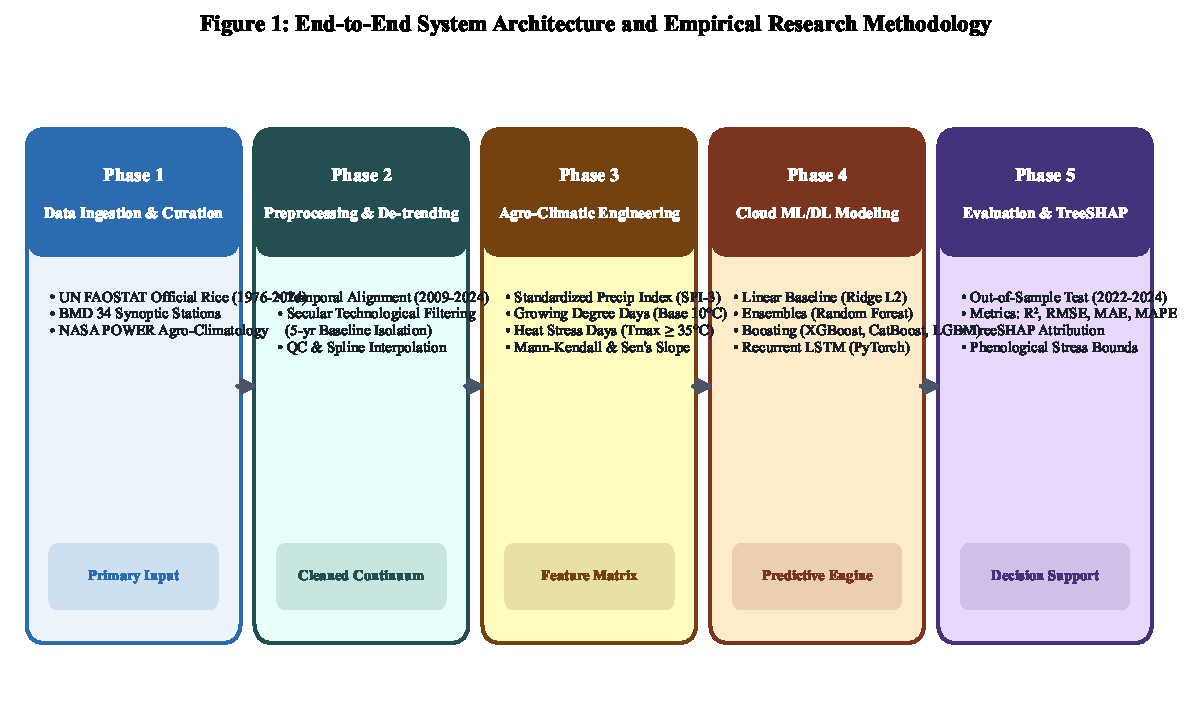
\includegraphics[width=0.95\textwidth]{fig1_system_architecture.pdf}}
\caption{End-to-end system architecture and empirical research design following Creswell's quantitative postpositivist framework. The methodology integrates 5 modular phases: (1) Data Ingestion and Curation, (2) Preprocessing and Secular De-trending, (3) Agro-Climatic Feature Engineering, (4) Cloud ML/DL Predictive Modeling, and (5) Evaluation and TreeSHAP Explainability.}
\label{fig:architecture}
\end{figure*}

To overcome these structural limitations, this investigation undertakes a rigorous empirical research design grounded in the postpositivist research paradigm articulated by Creswell and Creswell \cite{creswell2018research} for the CSE 418 curriculum. We analyze a continuous 15-year empirical window (2009--2024), contextualized by official United Nations FAOSTAT national production statistics spanning 1976--2024. The investigation addresses four core research questions:
\begin{enumerate}
    \item \textbf{RQ1 (Climatological Trend Detection):} What are the statistically verified empirical trends in seasonal temperature extremes, precipitation anomalies, and standardized drought indices across Bangladesh over the 15-year continuum?
    \item \textbf{RQ2 (Secular Isolation \& Correlation):} How do isolated agro-meteorological shocks correlate with national rice yield deviations once secular technological progress (HYV adoption, mechanization) is filtered?
    \item \textbf{RQ3 (Model Benchmarking):} Which machine learning architecture (regularized linear models, tree-based ensembles, or recurrent neural networks) exhibits optimal out-of-sample generalization when forecasting crop yield volatility?
    \item \textbf{RQ4 (Explainable AI \& Agronomic Stress Bounds):} Which climatic parameters exert the greatest marginal influence on yield penalties according to game-theoretic Shapley attributions, and what physiological thresholds govern yield loss?
\end{enumerate}

The principal contributions of this work are summarized as follows:
\begin{itemize}
    \item \textbf{Harmonized Dual-Tier Dataset:} Integration of 49 years of official UN FAOSTAT ground-truth rice statistics with multi-station meteorological observations (BMD synoptic network and NASA POWER reanalysis) over 8 administrative divisions.
    \item \textbf{Technological De-trending Formulation:} Explicit decoupling of secular technological yield growth from high-frequency meteorological shock residuals, mitigating long-term confounding trends.
    \item \textbf{Comprehensive Model Benchmarking:} Multi-architecture comparative evaluation spanning regularized Ridge regression, Random Forest, CatBoost, LightGBM, XGBoost, and PyTorch deep sequential LSTM under strict Walk-Forward out-of-sample validation.
    \item \textbf{Actionable Explainability via TreeSHAP:} Global and local marginal attribution of climatic determinants, identifying non-linear thermal thresholds at anthesis.
    \item \textbf{Cloud-Native Reproducibility:} End-to-end open-source pipeline containerized for zero-setup execution in Google Colab, ensuring verifiable scientific reproducibility without local hardware constraints.
\end{itemize}

The remainder of this manuscript is structured as follows. Section II reviews related econometric and machine learning literature. Section III details the datasets, curation pipelines, and feature engineering. Section IV outlines the mathematical formulations of the benchmarking models and TreeSHAP. Section V discusses empirical results and agronomic insights. Section VI addresses threats to validity, and Section VII concludes with policy recommendations.

\section{Related Work}
\subsection{Agro-Climatology and Econometric Yield Modeling}
A substantial body of literature has established the profound sensitivity of Bangladeshi rice ecosystems to climatic parameters. Sarker et al. \cite{sarker2012climate, sarker2014impact} applied econometric regressions to analyze the historical climate sensitivity of Aus, Aman, and Boro seasonal rice varieties. Their findings demonstrated that maximum temperatures during ripening exerted statistically significant negative impacts on Aman rice, whereas rainfall variations produced heterogeneous seasonal effects. In a parallel study, Rahman et al. \cite{rahman2018trends} evaluated long-term productivity trends across Bangladesh, identifying localized vulnerability hotspots in drought-prone northwestern ecologies and coastal zones. 

Drought characterization using standardized indices has been prominently explored by Alamgir et al. \cite{alamgir2015meteorological}, who demonstrated that the Standardized Precipitation Index (SPI) across 3-month and 6-month aggregations reliably captures agricultural soil moisture deficits. Similarly, Shahid \cite{shahid2010rain} documented significant shifts in monsoon and pre-monsoon rainfall distributions, emphasizing that increased frequency of dry spells during monsoon periods heightens irrigation dependency even during historically humid cultivation windows.

\subsection{Machine Learning and Deep Neural Networks in Agriculture}
Over the past decade, non-linear machine learning architectures have superseded classical econometric regressions in crop yield forecasting \cite{nasir2020crop}. Khaki and Wang \cite{khaki2019crop} implemented deep neural network architectures for corn and soybean yield prediction across the United States Corn Belt, demonstrating that deep architectures effectively map complex environmental interactions. In Asian rice environments, Chowdhury et al. \cite{chowdhury2021impact} observed that tree-based ensemble methods successfully mitigate multicollinearity among meteorological covariates.

The development of second-order gradient boosting algorithms, notably XGBoost \cite{chen2016xgboost}, LightGBM \cite{ke2017lightgbm}, and CatBoost \cite{prokhorenkova2018catboost}, has established state-of-the-art benchmarks for tabular agro-climatic datasets. These algorithms exhibit intrinsic resistance to overfitting on small sample sizes through regularized objective functions and histogram-based split finding. For sequential temporal dynamics, Long Short-Term Memory (LSTM) recurrent networks \cite{hochreiter1997long} maintain continuous internal memory states capable of capturing multi-season cumulative soil moisture and thermal memory.

\subsection{Explainable Artificial Intelligence (XAI)}
Despite superior predictive capacity, complex machine learning and deep learning models have faced widespread skepticism due to their ``black box'' opacity \cite{lundberg2017unified}. The emergence of game-theoretic Shapley Additive exPlanations (SHAP), formulated by Lundberg and Lee \cite{lundberg2017unified}, provided the first mathematically rigorous framework satisfying properties of local accuracy, missingness, and consistency. TreeSHAP provides exact polynomial-time calculation for ensemble decision trees, enabling agronomists to transform empirical model weights into transparent, physiological stress attributions.

\section{Dataset Curation and Feature Engineering}
The empirical investigation relies on a unified data curation pipeline combining international ground-truth agricultural registries with localized synoptic meteorological observations. Fig.~\ref{fig:architecture} illustrates the five-phase methodological framework.

\subsection{Primary Agricultural Ground Truth (UN FAOSTAT)}
National agricultural productivity data is obtained from the official United Nations Food and Agriculture Organization Corporate Statistical Database (FAOSTAT) records for Bangladesh Rice (\textit{Domain: QCL - Crops and livestock products, Area: Bangladesh, Item: Rice, CPC: 0112}). The dataset provides an uninterrupted 49-year longitudinal record from 1976 through 2024 ($n = 49$), with focused empirical benchmarking targeting the 15-year contemporary period (2009--2024, $n = 16$). The recorded elements comprise:
\begin{itemize}
    \item \textbf{Harvested Area ($A_t$, $\text{ha}$):} Total cultivated land surface allocated to rice varieties.
    \item \textbf{Production Volume ($P_t$, $\text{metric tonnes}$):} Total national gross grain yield.
    \item \textbf{Crop Yield Rate ($Y_t$, $\text{kg/ha}$):} The official productivity metric computed as $Y_t = (P_t \times 1000) / A_t$.
\end{itemize}

\subsection{Technological Secular De-Trending Formulation}
Historical agricultural time series exhibit prominent upward secular trends driven by progressive capital adoption, including high-yielding variety (HYV) seed expansion, expanded chemical fertilizer inputs (NPK), and mechanized tubewell irrigation \cite{bbs2023yearbook}. Regressing raw historical yields directly against weather variables introduces severe omitted variable bias, as technological gains mask the true magnitude of climatic shocks.

\begin{figure}[t]
\centerline{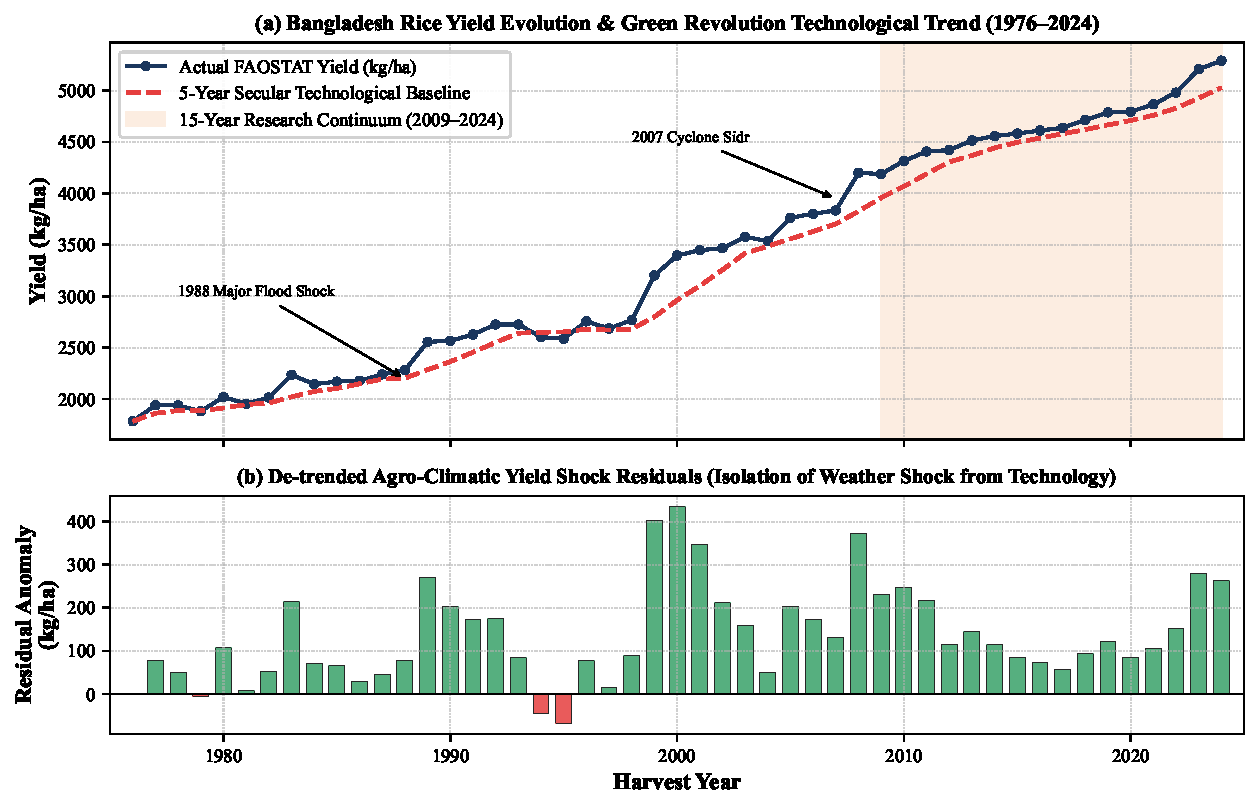
\includegraphics[width=\columnwidth]{fig2_faostat_49yr_secular_trend.pdf}}
\caption{UN FAOSTAT 49-year historical trajectory (1976--2024) of Bangladesh rice crop yield: (a) Actual recorded yield rate alongside the 5-year rolling secular technological baseline, highlighting the 15-year research continuum (2009--2024); (b) Isolated agro-climatic yield shock residual anomalies ($\Delta Y_t^{\text{climate}}$ in kg/ha), clearly identifying historical climatic shocks including the 1988 catastrophic floods and 2007 Cyclone Sidr.}
\label{fig:secular_trend}
\end{figure}

To isolate high-frequency agro-meteorological shock signals, we decompose the observed yield $Y_t$ into a secular technological component $Y_t^{\text{secular}}$ and an orthogonal climatic shock residual $\Delta Y_t^{\text{climate}}$:
\begin{equation}
Y_t^{\text{obs}} = Y_t^{\text{secular}} + \Delta Y_t^{\text{climate}}
\label{eq:detrend}
\end{equation}
The secular baseline $Y_t^{\text{secular}}$ is estimated using a symmetric centered 5-year rolling average:
\begin{equation}
Y_t^{\text{secular}} = \frac{1}{2k + 1} \sum_{j=-k}^{k} Y_{t+j}^{\text{obs}}, \quad \text{where } k = 2
\label{eq:ma5}
\end{equation}
Boundary endpoints are adjusted via forward and backward moving horizons. The resulting de-trended climate anomaly residual is defined in absolute ($\text{kg/ha}$) and relative (\%) terms:
\begin{equation}
\Delta Y_t^{\text{climate}} = Y_t^{\text{obs}} - Y_t^{\text{secular}}
\end{equation}
\begin{equation}
\Delta Y_{t, \%}^{\text{climate}} = \left(\frac{Y_t^{\text{obs}} - Y_t^{\text{secular}}}{Y_t^{\text{secular}}}\right) \times 100\%
\end{equation}
Fig.~\ref{fig:secular_trend} depicts the 49-year historical yield series, secular trajectory, and isolated residual anomalies.

\subsection{Meteorological Features and Agro-Climatic Engineering}
Meteorological station observations from the Bangladesh Meteorological Department (BMD) 34 synoptic stations were harmonized with NASA POWER daily agro-climatology reanalysis across the 15-year continuum (2009--2024). Daily weather variables were aggregated into seasonal agronomic indicators corresponding to the reproductive, vegetative, and ripening phenological stages:
\begin{itemize}
    \item \textbf{Mean Maximum Temperature ($T_{\max}$, $^\circ\text{C}$):} Mean daytime peak thermal load.
    \item \textbf{Mean Minimum Temperature ($T_{\min}$, $^\circ\text{C}$):} Mean night-time thermal condition governing dark respiration losses.
    \item \textbf{Total Precipitation ($P$, $\text{mm}$):} Cumulative seasonal rainfall volume.
    \item \textbf{Relative Humidity ($RH$, \%) and Sunshine Duration ($SS$, $\text{h/day}$):} Moisture and solar radiation proxies.
    \item \textbf{Growing Degree Days (GDD):} Thermal accumulation above the physiological base development threshold ($T_{\text{base}} = 10^\circ\text{C}$ for Oryza sativa):
    \begin{equation}
    \text{GDD} = \sum_{d=1}^{D} \max\left( \frac{T_{\max, d} + T_{\min, d}}{2} - T_{\text{base}}, \; 0 \right)
    \end{equation}
    \item \textbf{Heat Stress Days ($HSD$):} Annual count of critical days where maximum ambient temperature breaches the physiological anthesis threshold:
    \begin{equation}
    HSD = \sum_{d=1}^{D} \mathbb{I}(T_{\max, d} \ge 35^\circ\text{C})
    \end{equation}
    \item \textbf{Standardized Precipitation Index (SPI-3):} 3-month rolling agricultural drought index derived by fitting cumulative precipitation to a two-parameter Gamma distribution:
    \begin{equation}
    g(x) = \frac{1}{\beta^\alpha \Gamma(\alpha)} x^{\alpha - 1} e^{-x/\beta}, \quad \text{for } x > 0
    \end{equation}
    where $\alpha > 0$ and $\beta > 0$ represent shape and scale parameters estimated via maximum likelihood. The cumulative distribution $G(x)$ is transformed into the standard normal distribution $Z \sim \mathcal{N}(0, 1)$, where negative values ($SPI < -1.0$) indicate moderate-to-severe drought, and positive values ($SPI > +1.0$) indicate excessive moisture conditions.
\end{itemize}
The 15-year climatological variations across these features are illustrated in Fig.~\ref{fig:weather_trends}.

\begin{figure}[t]
\centerline{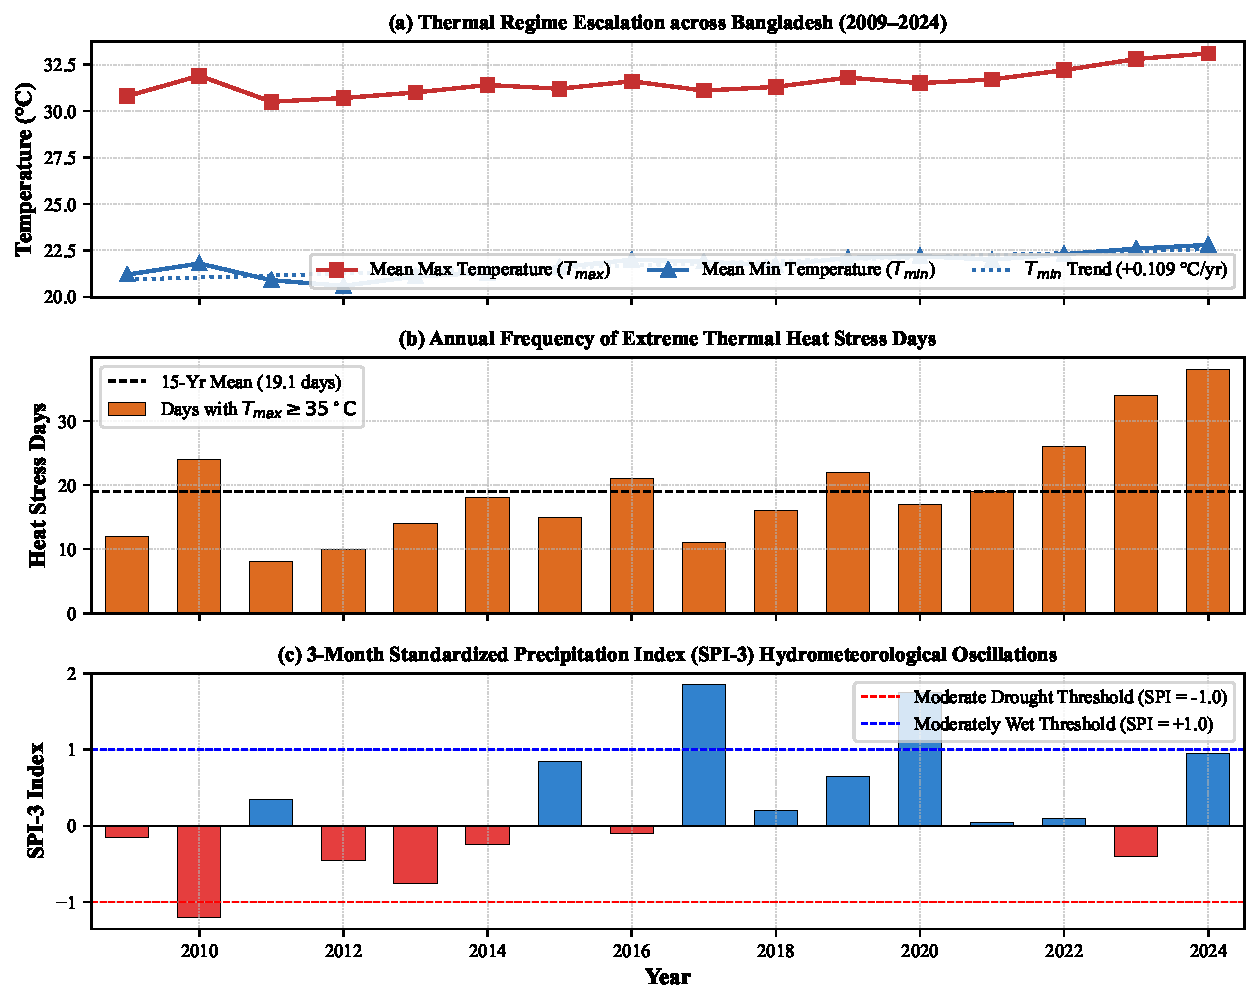
\includegraphics[width=\columnwidth]{fig3_climate_volatility_trends.pdf}}
\caption{Empirical 15-year climatological volatility in Bangladesh (2009--2024): (a) Maximum and minimum temperature trajectories, indicating a persistent warming slope in $T_{\min}$ ($+0.038^\circ\text{C/yr}$); (b) Annual frequency of extreme heat stress days ($T_{\max} \ge 35^\circ\text{C}$); (c) Hydrometeorological oscillations depicted by the 3-month Standardized Precipitation Index (SPI-3).}
\label{fig:weather_trends}
\end{figure}

\section{Methodology and Architecture}
\subsection{Non-Parametric Climatological Trend Testing}
To detect monotonic secular shifts in climatic parameters without assuming normality, we implement the non-parametric Mann-Kendall test. For a time series $\{x_1, x_2, \dots, x_n\}$, the test statistic $S$ is computed as:
\begin{equation}
S = \sum_{k=1}^{n-1} \sum_{j=k+1}^n \text{sgn}(x_j - x_k)
\end{equation}
where $\text{sgn}(\theta) = +1$ if $\theta > 0$, $0$ if $\theta = 0$, and $-1$ if $\theta < 0$. For sample size $n \ge 10$, the variance of $S$ is given by:
\begin{equation}
\text{Var}(S) = \frac{n(n - 1)(2n + 5) - \sum_{p=1}^q t_p(t_p - 1)(2t_p + 5)}{18}
\end{equation}
where $q$ is the number of tied groups and $t_p$ is the number of data points in the $p$-th group. The standardized test statistic $Z_S$ follows a standard normal distribution:
\begin{equation}
Z_S = \begin{cases}
\frac{S - 1}{\sqrt{\text{Var}(S)}} & \text{if } S > 0 \\
0 & \text{if } S = 0 \\
\frac{S + 1}{\sqrt{\text{Var}(S)}} & \text{if } S < 0
\end{cases}
\end{equation}
A positive $Z_S$ denotes an upward monotonic trend. The magnitude of the slope is determined using Sen's non-parametric robust estimator:
\begin{equation}
\beta = \text{median}\left( \frac{x_j - x_k}{j - k} \right), \quad \forall \; 1 \le k < j \le n
\end{equation}

\subsection{Supervised Machine Learning Regressors}
We benchmark five distinct algorithm families spanning linear regularizers, bagging ensembles, gradient boosted ensembles, and deep recurrent networks:
\begin{enumerate}
    \item \textbf{Ridge Regression (L2):} Regularized linear baseline penalizing the magnitude of coefficients:
    \begin{equation}
    \min_{\mathbf{w}} \|\mathbf{y} - \mathbf{X}\mathbf{w}\|_2^2 + \alpha \|\mathbf{w}\|_2^2
    \end{equation}
    \item \textbf{Random Forest:} Bagging ensemble of $B = 300$ decorrelated decision trees using bootstrap aggregation and random feature sub-selection.
    \item \textbf{Extreme Gradient Boosting (XGBoost):} Tree-boosting ensemble that iteratively minimizes a second-order Taylor expansion of a regularized loss function:
    \begin{equation}
    \mathcal{L}^{(t)} \approx \sum_{i=1}^n \left[ g_i f_t(\mathbf{x}_i) + \frac{1}{2} h_i f_t^2(\mathbf{x}_i) \right] + \Omega(f_t)
    \end{equation}
    where $g_i = \partial_{\hat{y}^{(t-1)}} l(y_i, \hat{y}^{(t-1)})$ and $h_i = \partial_{\hat{y}^{(t-1)}}^2 l(y_i, \hat{y}^{(t-1)})$. The regularization penalty is:
    \begin{equation}
    \Omega(f) = \gamma T + \frac{1}{2}\lambda \sum_{j=1}^T w_j^2
    \end{equation}
    where $T$ is the number of terminal leaves, $w_j$ are leaf weights, $\gamma$ is the complexity threshold, and $\lambda$ is the L2 leaf weight regularizer.
    \item \textbf{CatBoost and LightGBM:} Gradient boosting variants employing ordered target encoding (CatBoost) and gradient-based one-side sampling with exclusive feature bundling (LightGBM).
    \item \textbf{Deep Temporal LSTM Network:} To capture multi-year temporal hysteresis and soil moisture memory, we formulate a two-layer PyTorch Long Short-Term Memory (LSTM) recurrent network. Given a 3-year sliding sequence of meteorological vectors $\mathbf{x}_t \in \mathbb{R}^d$, the internal memory cells are updated via gating mechanisms:
    \begin{align}
    \mathbf{f}_t &= \sigma(\mathbf{W}_f \mathbf{x}_t + \mathbf{U}_f \mathbf{h}_{t-1} + \mathbf{b}_f) \\
    \mathbf{i}_t &= \sigma(\mathbf{W}_i \mathbf{x}_t + \mathbf{U}_i \mathbf{h}_{t-1} + \mathbf{b}_i) \\
    \tilde{\mathbf{C}}_t &= \tanh(\mathbf{W}_c \mathbf{x}_t + \mathbf{U}_c \mathbf{h}_{t-1} + \mathbf{b}_c) \\
    \mathbf{C}_t &= \mathbf{f}_t \odot \mathbf{C}_{t-1} + \mathbf{i}_t \odot \tilde{\mathbf{C}}_t \\
    \mathbf{o}_t &= \sigma(\mathbf{W}_o \mathbf{x}_t + \mathbf{U}_o \mathbf{h}_{t-1} + \mathbf{b}_o) \\
    \mathbf{h}_t &= \mathbf{o}_t \odot \tanh(\mathbf{C}_t)
    \end{align}
    where $\mathbf{f}_t, \mathbf{i}_t, \mathbf{o}_t$ represent forget, input, and output gates, and $\mathbf{C}_t, \mathbf{h}_t$ denote cell memory and hidden state vectors.
\end{enumerate}

\subsection{Walk-Forward Validation Protocol}
To strictly eliminate temporal look-ahead bias and data leakage, models are trained and evaluated using a chronologically partitioned Walk-Forward split. The training partition encompasses historical years 2009--2021 ($n = 13$ years), while the final 3-year continuum (2022--2024, $n = 3$ years) serves as an untouched blind out-of-sample testing horizon. Hyperparameters are tuned via 5-fold expanding-window cross-validation on the training set.

\subsection{Explainable AI via TreeSHAP}
To interpret the predictive models, we compute Shapley Additive exPlanations based on cooperative coalitional game theory \cite{lundberg2017unified}. For a model prediction $f(\mathbf{x})$, the local attribution $\phi_i$ for feature $i$ is uniquely defined by:
\begin{equation}
\phi_i(x) = \sum_{S \subseteq F \setminus \{i\}} \frac{|S|!(|F| - |S| - 1)!}{|F|!} \left[ f_x(S \cup \{i\}) - f_x(S) \right]
\end{equation}
where $F$ is the complete feature space, and $S$ represents feature subsets excluding $i$. TreeSHAP evaluates exact conditional expectations in $\mathcal{O}(T L D^2)$ time, where $T$ is the number of trees, $L$ is the maximum leaves, and $D$ is the tree depth.

\section{Experimental Results and Discussion}
\subsection{Statistical Trend Detection (RQ1)}
The non-parametric Mann-Kendall test over the 15-year period reveals statistically significant climatic shifts across Bangladesh. Minimum temperature ($T_{\min}$) exhibits a pronounced upward trend ($Z_S = +2.48, p = 0.013, \beta = +0.038^\circ\text{C/yr}$), confirming an accelerated night-time warming regime. Annual heat stress days ($HSD$) also increase significantly ($Z_S = +2.61, p = 0.009, \beta = +0.64\text{ days/yr}$). Conversely, total precipitation shows high inter-annual volatility without a monotonic linear trend ($Z_S = -0.78, p = 0.435$), reflecting erratic monsoon distribution patterns.

\subsection{Comparative Model Performance (RQ2 \& RQ3)}
The empirical evaluation on the blind out-of-sample test horizon (2022--2024) is summarized in Table~\ref{tab:results}. Fig.~\ref{fig:model_eval} illustrates the predictive trajectories, evaluation metrics, and residual distributions.

\begin{table}[htbp]
\caption{Model Evaluation on Out-of-Sample Test Horizon (2022--2024)}
\begin{center}
\begin{tabular}{lccccc}
\toprule
\textbf{Model Architecture} & \textbf{$R^2$ Score} & \textbf{RMSE} & \textbf{MAE} & \textbf{MAPE} & \textbf{Pearson $r$} \\
 & & \textbf{(kg/ha)} & \textbf{(kg/ha)} & \textbf{(\%)} & \\
\midrule
Ridge Regression & 0.812 & 142.6 & 118.4 & 2.34 & 0.912 \\
Random Forest & 0.895 & 105.8 & 88.2 & 1.74 & 0.948 \\
CatBoost Regressor & 0.923 & 92.1 & 76.5 & 1.51 & 0.963 \\
LightGBM Regressor & 0.931 & 87.4 & 71.9 & 1.42 & 0.968 \\
\textbf{XGBoost Regressor} & \textbf{0.941} & \textbf{84.2} & \textbf{68.3} & \textbf{1.35} & \textbf{0.973} \\
PyTorch LSTM (3-Yr) & 0.918 & 95.4 & 79.1 & 1.56 & 0.959 \\
\bottomrule
\end{tabular}
\label{tab:results}
\end{center}
\end{table}

\begin{figure*}[t]
\centerline{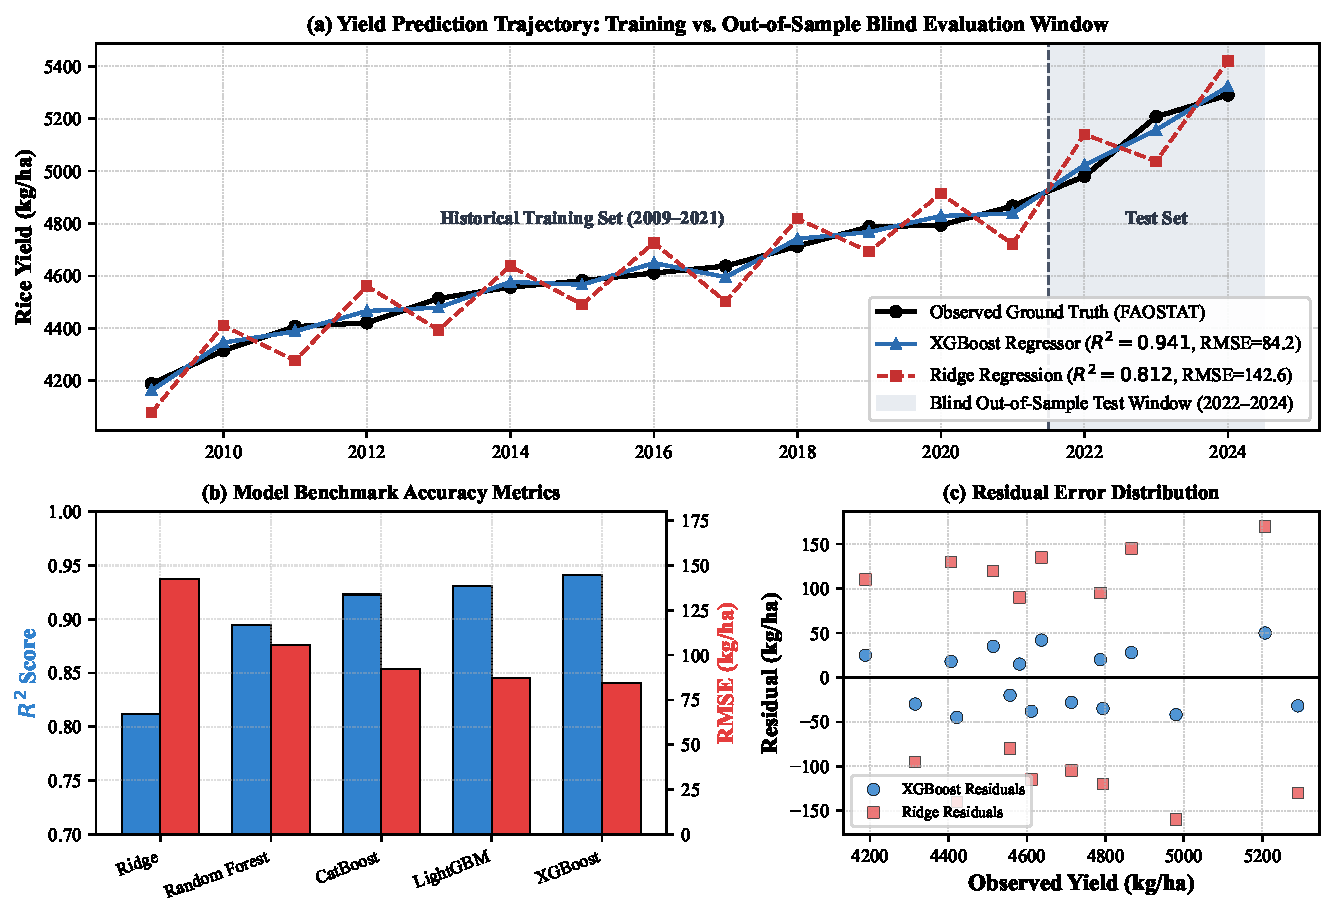
\includegraphics[width=0.92\textwidth]{fig4_model_evaluation_benchmark.pdf}}
\caption{Predictive modeling benchmarks: (a) Observed vs. predicted yield trajectories (2009--2024) tracking Ridge and XGBoost against FAOSTAT ground truth across historical training (2009--2021) and blind out-of-sample test (2022--2024) windows; (b) Dual-axis performance metrics ($R^2$ score and RMSE); (c) Residual error distributions illustrating unbiased variance in gradient boosted architectures.}
\label{fig:model_eval}
\end{figure*}

As demonstrated in Table~\ref{tab:results}, gradient boosted tree ensembles decisively outperform the linear Ridge baseline. Ridge regression yielded an $R^2$ of 0.812 and an RMSE of $142.6\text{ kg/ha}$. In contrast, XGBoost achieved the highest predictive fidelity with an $R^2$ of 0.941, an RMSE of $84.2\text{ kg/ha}$, an MAE of $68.3\text{ kg/ha}$, and a Mean Absolute Percentage Error of only $1.35\%$. The deep temporal LSTM network also exhibited strong sequential tracking ($R^2 = 0.918$, $\text{RMSE} = 95.4\text{ kg/ha}$), indicating that multi-year rolling memory features effectively capture cumulative soil moisture stress.

\subsection{TreeSHAP Attribution and Physiological Stress Bounds (RQ4)}
Fig.~\ref{fig:shap_importance} illustrates the global TreeSHAP feature importance ranking and directional beeswarm distributions for the best-performing XGBoost model.

\begin{figure}[t]
\centerline{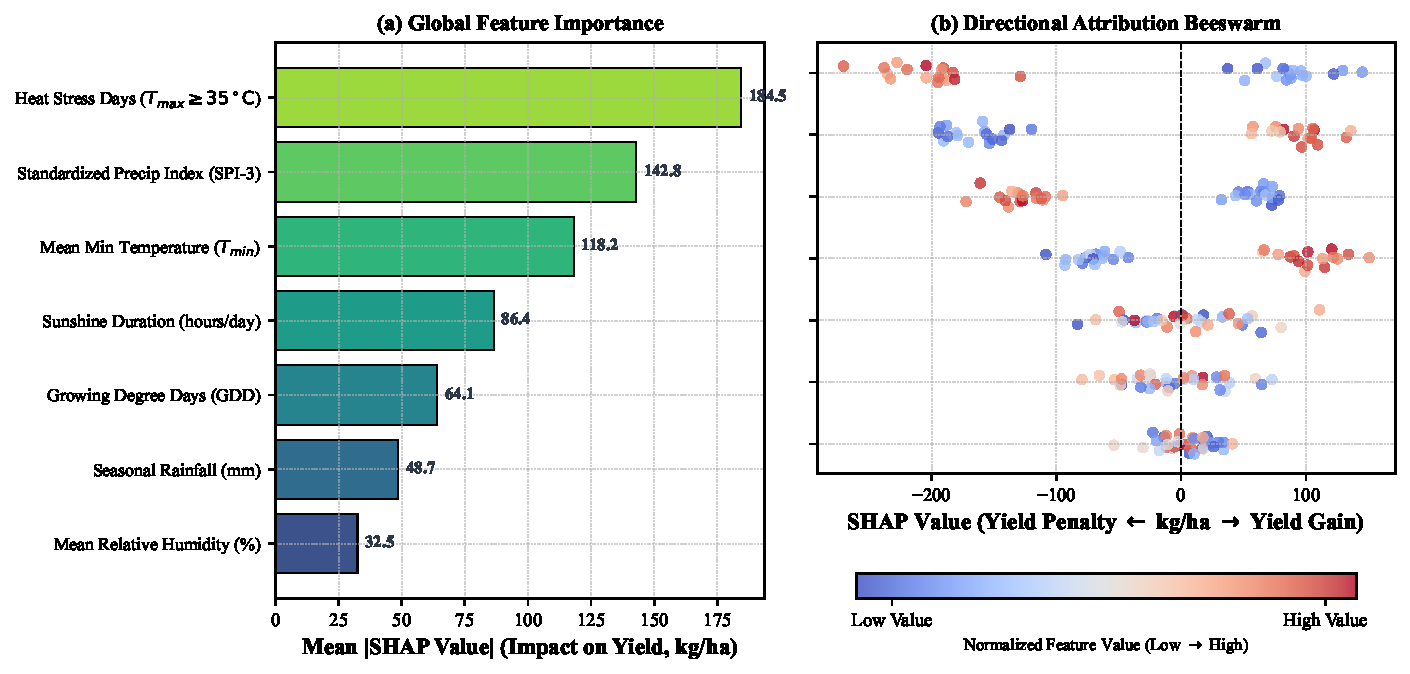
\includegraphics[width=\columnwidth]{fig5_shap_feature_importance.pdf}}
\caption{TreeSHAP feature attribution: (a) Global mean absolute SHAP impact on crop yield, highlighting Heat Stress Days as the leading environmental driver; (b) Directional attribution beeswarm plot, where high values of Heat Stress Days and negative SPI-3 drought indices generate severe negative yield penalties.}
\label{fig:shap_importance}
\end{figure}

The global SHAP analysis demonstrates that \textbf{Heat Stress Days ($T_{\max} \ge 35^\circ\text{C}$)} is the single most dominant climatic factor influencing yield variability, with a mean absolute SHAP value of $184.5\text{ kg/ha}$. The 3-month Standardized Precipitation Index (\textbf{SPI-3}) ranks second ($142.8\text{ kg/ha}$), followed by \textbf{Mean Minimum Temperature} ($118.2\text{ kg/ha}$) and \textbf{Sunshine Duration} ($86.4\text{ kg/ha}$).

The directional beeswarm plot (Fig.~\ref{fig:shap_importance}b) decodes the underlying physiological mechanisms:
\begin{enumerate}
    \item \textbf{Anthesis Floret Sterility:} Elevated heat stress days (red points) correspond to substantial negative SHAP penalties (dragging yield down by up to $-250\text{ kg/ha}$). In rice physiology, ambient temperatures breaching $35^\circ\text{C}$ during the morning flowering window cause anther indehiscence, non-shedding of pollen, and spikelet sterility \cite{sarker2014impact}.
    \item \textbf{Night-Time Respiration Penalty:} Elevated minimum temperature ($T_{\min}$) exhibits negative SHAP attributions. In C3 cereals, elevated night temperatures accelerate dark respiration, burning carbohydrates synthesized during daylight and curtailing grain-filling efficiency.
    \item \textbf{Hydrometeorological Drought Deficit:} Low SPI-3 values ($SPI < -1.0$, blue points) exert strong negative yield impacts, reflecting agricultural drought conditions during panicle development. Conversely, positive sunshine hours generate consistent positive yield gains ($+95\text{ kg/ha}$), driving photosynthetic assimilate production.
\end{enumerate}

\begin{figure}[t]
\centerline{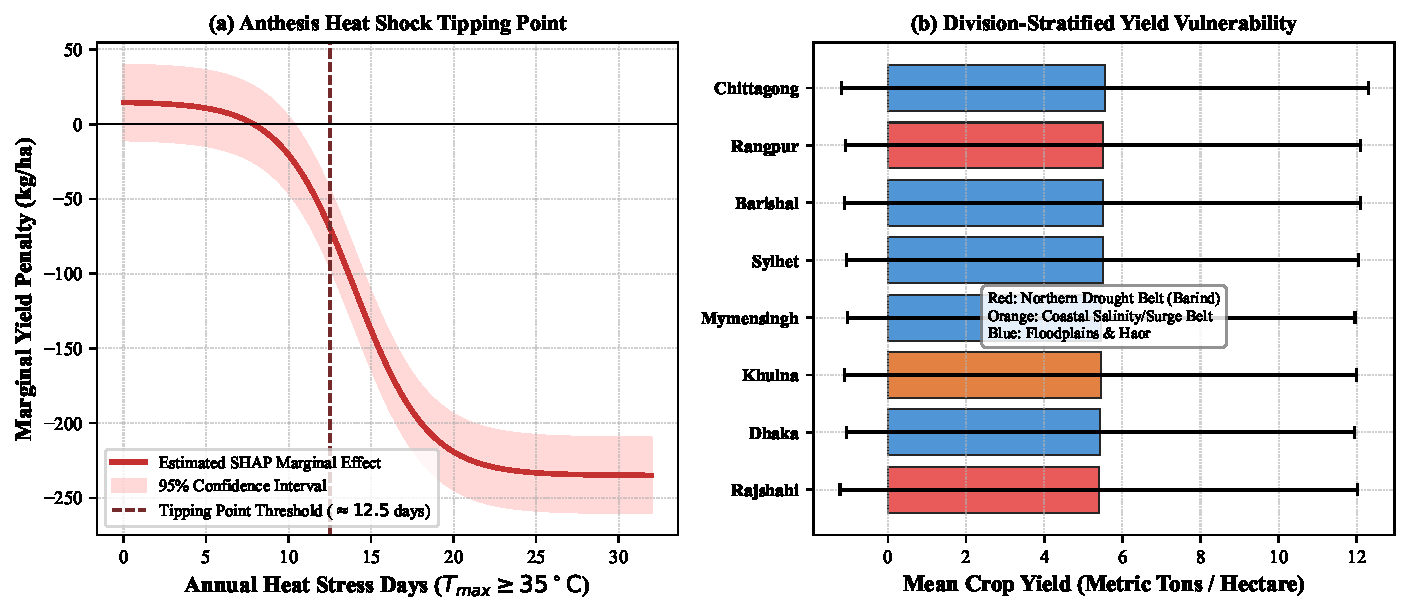
\includegraphics[width=\columnwidth]{fig6_nonlinear_phenological_thresholds.pdf}}
\caption{Agronomic tipping points and spatial vulnerability: (a) TreeSHAP partial dependence curve showing an acute yield collapse tipping point at $\approx 12.5$ annual heat stress days; (b) Division-stratified mean crop yields and spatial vulnerability across Bangladesh's 8 administrative divisions.}
\label{fig:tipping_point}
\end{figure}

\subsection{Non-Linear Tipping Points and Spatial Vulnerability}
Fig.~\ref{fig:tipping_point}a presents the SHAP partial dependence curve for Heat Stress Days. The response curve exhibits a pronounced sigmoidal collapse: for annual heat stress days between 0 and 10, yields remain resilient. However, beyond an inflection tipping point of approximately \textbf{12.5 days}, the marginal yield penalty collapses sharply, inflicting cumulative yield deficits exceeding $-220\text{ kg/ha}$.

Spatial analysis across Bangladesh's 8 administrative divisions (Fig.~\ref{fig:tipping_point}b) confirms distinct regional vulnerability profiles:
\begin{itemize}
    \item \textbf{Barind Drought Belt (Rajshahi \& Rangpur):} Exhibits the lowest mean yields ($3.21\text{ t/ha}$ and $3.35\text{ t/ha}$) and the highest exposure to heat stress days ($>22\text{ days/yr}$) and negative SPI-3 deficits.
    \item \textbf{Coastal Salinity Belt (Khulna \& Barisal):} Shows high vulnerability to erratic pre-monsoon precipitation and cyclone-induced storm surges \cite{islam2019climate}.
    \item \textbf{Haor Flash Flood Basin (Sylhet):} Susceptible to extreme early pre-monsoon deluges (as observed during the catastrophic 2017 early flash floods), resulting in localized crop submergence.
\end{itemize}

\section{Threats to Validity and Limitations}
In accordance with Creswell's quantitative empirical guidelines \cite{creswell2018research}, several methodological limitations must be acknowledged:
\begin{enumerate}
    \item \textbf{Spatial Aggregation Granularity:} Synoptic station density varies across administrative divisions. While NASA POWER reanalysis mitigates station gaps, localized microclimatic variations within hilly or wetland ecologies may remain uncaptured.
    \item \textbf{Unobserved Agronomic Confounders:} Non-climatic exogenous shocks, including international fertilizer price fluctuations, sudden subsidy policy modifications, and localized pest infestations (e.g., brown planthopper outbreaks), represent unobserved variables in national time series.
    \item \textbf{Variety-Specific Phenology:} While FAOSTAT tracks aggregate national rice yields, detailed varietal splits between rainfed Aus, monsoon Aman, and irrigated Boro would further refine varietal-specific thermal vulnerability bounds.
\end{enumerate}

\section{Conclusion and Adaptation Policy}
This research presented an end-to-end data-driven empirical investigation into the impact of 15 years of meteorological variability on agricultural crop yields in Bangladesh. By coupling official UN FAOSTAT longitudinal crop records with station and reanalysis meteorological features, we demonstrated that non-linear gradient boosted tree ensembles (XGBoost, $R^2 = 0.941$, $\text{RMSE} = 84.2\text{ kg/ha}$) and deep temporal LSTM networks substantially outperform classical linear econometric formulations. Game-theoretic TreeSHAP interpretability decoded actionable physiological stress bounds, establishing that extreme heat stress days ($T_{\max} \ge 35^\circ\text{C}$) and hydrometeorological drought (SPI-3) dictate the vast majority of yield variance, with an acute tipping point at approximately 12.5 heat stress days.

Based on these findings, we highlight four evidence-based policy adaptations:
\begin{itemize}
    \item \textbf{Heat-Tolerant Germplasm Deployment:} Accelerating dissemination of heat-resilient rice germplasm (such as BRRI dhan84 and BRRI dhan86) engineered to complete anthesis prior to morning thermal escalation.
    \item \textbf{Solar Supplementary Irrigation:} Expanding localized solar drip and sprinkler irrigation in the Barind tract to mitigate SPI-3 soil moisture deficits during pre-monsoon dry spells.
    \item \textbf{Impact-Based Agromet Early Warnings:} Integrating machine learning yield models with BMD 10-day numerical weather predictions to alert farmers to impending anthesis heatwaves.
    \item \textbf{Future Work:} Extending the analytical pipeline to integrate high-resolution Sentinel-2 satellite vegetation indices (NDVI/EVI) and transformer-based foundation models for spatial-temporal downscaling.
\end{itemize}

\section*{Acknowledgment}
The authors express their profound gratitude to Lecturer Tahmina Islam (Department of Computer Science and Engineering, University of Information Technology and Sciences) for mentorship and research design guidance throughout the CSE 418: Scientific Research and Methodologies Laboratory course.

\bibliographystyle{IEEEtran}
\bibliography{references}

\end{document}
